\documentclass[a4paper]{article}
\usepackage{geometry}
\geometry{a4paper, portrait, margin=1in}
\usepackage[english]{babel}
\usepackage[utf8]{inputenc}
\usepackage{natbib}
\usepackage{graphicx}
\usepackage{fancyhdr}
\usepackage{array}
\usepackage{tabu}
\usepackage{listings}

\title{Computing GCSE Coursework}
\author{\\ \\ \\ \\ Thomas Bass\\Candidate 4869\\Centre 52423\\OCR A453 Programming Project\\\\Made with \LaTeX}
\date{2016-2017}


\pagestyle{fancy}
\fancyhf{}
\rhead{Computing GCSE Coursework}
\chead{Candidate 4869}
\lhead{Thomas Bass}
\rfoot{Page \thepage}

\begin{document}

\maketitle
\pagebreak
\renewcommand*\contentsname{Summary}
\tableofcontents
\pagebreak
%%%%%%%%%%%%%%%%%%%%%%%%%%%%%%%%%%%%%%%%%%%%%%%%%%%%%%%%%%%%%%%%%%%%%%%%%%%%
\section{Objectives}

\subsection{Task 1}
\begin{enumerate}
\item{Take an input and verify that it is 8 or 7 numerical digits}
\item{Calculate the 8th check digit:}
\item[~a]{Multiply the first 7 numbers alternately by 3,1}
\item[~b]{Total these results}
\item[~c]{Subtract this sum from its nearest highest multiple of 10}
\item{Compare this to the given 8th number, or complete the 7-digit number}
\end{enumerate}

\subsection{Task 2}
\begin{enumerate}
\item{Take an input and validate that it is 8 numerical digits}
\item{Connect to a SQL database and run a query}
\item{Collect and display the results}
\item{Update the database with the customer?s order}
\item{Print a receipt}
\item{Cope with SQL errors}
\end{enumerate}

\subsection{Task 3}
\begin{enumerate}
\item{Scan a database and find stock to order}
\item{Create a receipt of the order}
\item{Update the database with the updated stock level}
\item{Cope with any SQL errors}
\end{enumerate}

\pagebreak

%%%%%%%%%%%%%%%%%%%%%%%%%%%%%%%%%%%%%%%%%%%%%%%%%%%%%%%%%%%%%%%%%%%%%%%%%%%%
\section{Test Plan}

\subsection{Task 1}
\begin{enumerate}
\item{Input strings of incorrect length. If rejected, it passes.}
\item[~]{Test data: \verb|12345|}
\item[~]{Test data: \verb|1234567890|}
\item{Input strings of letters. If rejected, it passes.}
\item[~]{Test data: \verb|abcdefg|}
\item{Get program to run a valid input. Print out totals at each stage, and check them manually. If they are the same, it passes.}
\item[~]{Test data: \verb|13245627|}
\item[~i.]{Manually add the totals of a valid input. If they are the same, it passes.}
\item[~ii.]{Manually round the total to the highest 10. If it is the same, it passes.}
\item[~iii.]{Manually collect the distance rounded. If it is the same, it passes.}
\item{Run the program with a GTIN number taken from a product. If it correctly calculated and verified, it passes.}
\end{enumerate}

\subsection{Task 2}
\begin{enumerate}
\item{Input strings of incorrect length. If rejected, it passes.}
\item[~]{Test data: \verb|12345|.}
\item[~]{Test data: \verb|1234567890|.}
\item{Input strings of letters. If rejected, it passes.}
\item[~]{Test data: \verb|abcdefg|.}
\item{Input a valid string to search. If product found, it passes.}
\item[~]{Test data: \verb|11440529|.}
\item{Manually check that the program has displayed the correct stock level and information. If it does, it passes.}
\item[~]{Stock info: 50 in stock for \#\verb|11440529| (red paint 100ml).}
\item{Order a quantity of the product. If the program updates the stock levels, it passes.}
\item[~]{Test data: order 5 x QTY of \#\verb|11440529| (red paint 100ml).}
\item{Complete a full order. If the program displays a receipt with the correct values, it passes.}
\item[~]{Test data: order 5 x QTY of \#\verb|11440529| (red paint 100ml) AND}
\item[~]{6 x QTY of \#\verb|11509493| (blue paint 100ml).}
\item[~]{Expected result: 5 x \#\verb|11509493| = \pounds9.95 AND 6x \#\verb|11509493| = \pounds11.94, total:  \pounds21.90 .}
\item{Provide the program with invalid values (such as ordering negative values). If the program rejects these, it passes.}
\item[~]{Test data: -3 x QTY \#\verb|11509493|.}
\item[~]{Expected result: error and re-input.}
\item[~]{Test data 0 x QTY \#\verb|11509493|.}
\item[~]{Expected result: error and re-input.}
\item[~]{Test data: 100 x QTY \#\verb|11509493|.}
\item[~]{Expected result: not enough stock, re-input.}
\end{enumerate}

\subsection{Task 3}
\begin{enumerate}
\item{Edit database for reduced stock. If reduced stock is identified, it passes.}
\item[~]{Test data: Edit a stock level to -10 of stock level.}
\item[~]{Print receipt.}
\item{Edit database for reduced stock. If a human-readable receipt is produced, it passes.}
\item[~]{Test data: Edit two stock levels to -10 of stock level.}
\item[~]{Print receipt.}
\item{Complete order for reduced stock. If the database updated, it passes.}
\item[~]{Continue from test area 2, and update database.}
\item[~]{Check database manually.}
\item{If the program handles SQL errors, it passes.}
\item[~]{Attempt to update from more than stock level.}
\end{enumerate}


\pagebreak

%%%%%%%%%%%%%%%%%%%%%%%%%%%%%%%%%%%%%%%%%%%%%%%%%%%%%%%%%%%%%%%%%%%%%%%%%%%%
\section{Pseudocode}
\subsection{Task 1}
\begin{lstlisting}
START
User INPUT choice for calculate or verify	
IF Calculate:
Number Length is 7
  INPUT GTIN
  CALL Verify function
ELSE IF Verify:
  Number Length is 8
  INPUT GTIN
  CALL verify Function
ENDIF
ENDIF
Verify Function:
  IF GTIN length = Length AND is all numeric:
    For a loop of 7 by step of 2:
      total = total+(GTIN [counter]*3)
      IF counter =6:
        Round total UP to nearest multiple of 10
        result = roundedNumber - total
          If Length = 7:
            Print result
          ELSE
            If GTIN at position Length = result:
              Print GTIN is a valid number
            ELSE:
              Print GTIN is an invalid number
            ENDIF
      ELSE
        Multiply GTIN at position of counter+1 by 1 and add to total
      ENDIF
  ELSE
    Print error and return to GTIN input
  ENDIF
END
\end{lstlisting}
\pagebreak

\subsection{Task 2}
\begin{lstlisting}
START
User INPUT GTIN number
IF GTIN is numerical AND GTIN = 8 charachters:
  Search Database for GTIN number
  IF result found:
    User INPUT quantity to order
    IF quantity > 0 AND quantity <= stock available
      PRINT receipt with total cost (cost per item * quantity ordered)
      Update Database with new stock (stock available a quantity ordered)
      User INPUT choice to order more items
      IF choice = yes:
        Add to order list and return to GTIN INPUT
      ELSE
        PRINT final receipt (order list) and end program
      ENDIF
    ELSE
      Return to Quantity INPUT
    ENDIF
  ELSE
    Return to GTIN INPUT
  ENDIF
ELSE
  Return to GTIN INPUT	
ENDIF
END
\end{lstlisting}
\

\subsection{Task 3}
\begin{lstlisting}
START
Connect to SQL Database
Search database:
  IF stock level < target stock level:
  RETURN results
PRINT results
APPEND results to order list
IF order complete:
  UPDATE database:
  stock level = target stock level
ELSE
  END
ENDIF
END
\end{lstlisting}

\pagebreak

%%%%%%%%%%%%%%%%%%%%%%%%%%%%%%%%%%%%%%%%%%%%%%%%%%%%%%%%%%%%%%%%%%%%%%%%%%%%

\section{Data Structure}
\subsection{Task 1}
\begin{center}
\begin{tabular}{ | m{13em} | m{16em} | }
  \hline
  Variable Name & Variable Description	\\ [0.5ex] 
  \hline\hline
  \verb|ask| & The choice wether the user wants to verify or calculate \\
  \hline
  \verb|gtin| & The GTIN number used \\
  \hline
  \verb|length| & The length the GTIN should be \\
  \hline
  \verb|total| & The running total of all the multiplications \\
  \hline
  \verb|checkdig| & The 8th digit in a verification \\
  \hline
  \verb|rounded| & \verb|total| Rounded up to the nearest 10 \\ 
  \hline
  \verb|result| & The 8th digit as the program calculates it \\
  \hline
  \verb|again| & The choice of wether the user wants to run the program again \\
  \hline 
\end{tabular}
\end{center}

\subsection{Task 2}
\begin{center}
\begin{tabular}{ | m{13em} | m{16em}| m{14em} | } 
 \hline
 Variable Name & Variable Description & Value \\ [0.5ex] 
 \hline\hline
 \verb|con| and \verb|cur| & Connections to SQL database & N/A \\ 
 \hline
 \verb|var| & User Input GTIN number & User Defined \\
 \hline
 \verb|results| & Fetchall results from SQL query & N/A (list) \\
 \hline
 \verb|product| & Equal to \verb|results|, reformatted & Equal to \verb|results| \\
 \hline
 \verb|sizeName| and \verb|sizeNameRaw| & Variables used to format the name of the product & Name of product selected \\
 \hline
 \verb|QtyToOrder| & User Input quantity ordered & User Defined \\
 \hline
 \verb|NewStockAvab| & Variable used to update the SQL database with the new stock levels & Stock Available minus \verb|QtyToOrder| \\ 
 \hline
 \verb|costOfOrder| & Total cost of order & Price of product*\verb|QtyToOrder| \\
 \hline
 \verb|currentOrderAddRaw| and \verb|currentOrderAdd| and \verb|currentOrder| & Variables used to format and append the order to the entire list of order (to print receipt) & N/A \\ [1ex] 
 \hline
\end{tabular}
\end{center}

\subsection{Task 3}
\begin{center}
\begin{tabular}{ | m{13em} | m{16em}| m{14em} | } 
  \hline
  Variable Name & Variable Description & Value \\ [0.5ex] 
  \hline\hline
  \verb|con| and \verb|cur| & Connections to SQL database & N/A \\
  \hline
  \verb|sql1| & SQL command for finding reduced stock levels & \verb|SELECT* FROM Inventory| \verb|WHERE StockAvab !=| \verb|Target Stock| \\
  \hline
  \verb|results| & Fetchall results from SQL query & N/A, List	\\
  \hline
  \verb|toOrder| & Value of how much stock needs to be ordered for each product & \verb|targetStock| - \verb|stockAvab| \\
  \hline
  \verb|sizeName| and \verb|sizeNameRaw| & Used to correctly format the product name & N/A \\
  \hline
  \verb|stockOrderAddRaw| and \verb|stockOrderAdd| and \verb|stockOrder| & Used to format the list of the stock update order & N/A \\
  \hline
  \verb|orderList| & Final order list & N/A \\
  \hline
  \end{tabular}
\end{center}

%%%%%%%%%%%%%%%%%%%%%%%%%%%%%%%%%%%%%%%%%%%%%%%%%%%%%%%%%%%%%%%%%%%%%%%%%%%%

\section{Development}
\subsection{Task 1}
\paragraph{Objective 1: Take an input and verify that it is 8 or 7 numerical digits}
\subparagraph{\texttt{start()} Function} ~ \par ~ \par
\noindent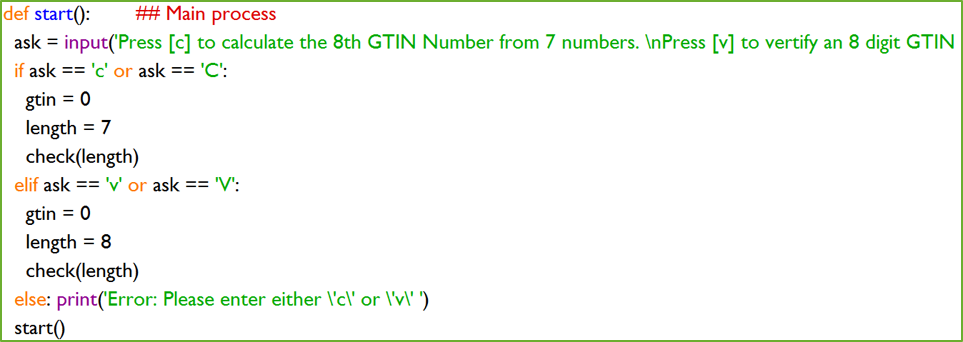
\includegraphics{task1_start()function.png}
This function takes a user input of 'ask' to decide if the user wants to either calculate the 8th GTIN digit from 7 digits (choice \verb|c|), or verify the 8th GTIN digit from 8 digits (choice \verb|v|). 
If the choice is \verb|c|, the program creates the variables \verb|gtin| and \verb|length|, and sets \verb|length| to 7. It then calls the \verb|check()| function carrying \verb|length| with it. \par
If the choice is \verb|v|, the program creates the variables \verb|gtin| and \verb|length|, and sets \verb|length| to 8. It then calls the \verb|check()| function carrying \verb|length| with it.
\par
\subparagraph{\texttt{check()} Function} ~ \par ~ \par
\noindent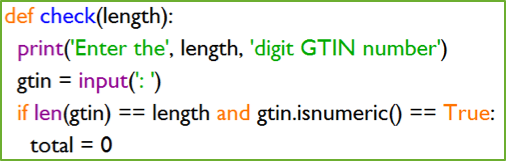
\includegraphics{task1_check()function2.png} ~ \par
\noindent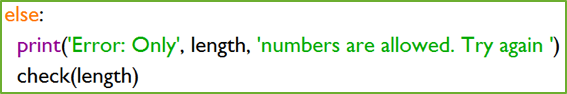
\includegraphics{task1_check()function3.png} ~\par
This function prints a statement asking the user for the \verb|length| length GTIN. It then takes the user input of \verb|gtin|. \par
If the length of \verb|gtin| is equal to \verb|length| and \verb|gtin.isnumeric| function is True (the variable is numerical) then it creates the variable \verb|total|. Else, it prints an error message, and returns to the \verb|check()| function.
\newpage

\paragraph{Objective 2: Calculate the 8th check digit}
\subparagraph{Multiply the first 7 numbers alternately by 3,1} ~ \par ~ \par
\noindent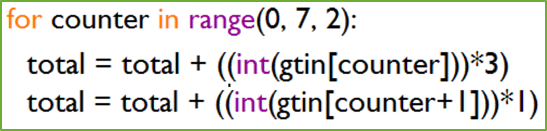
\includegraphics{task1_multiply1.png} ~\par
This snippet starts a loop for the value of \verb|counter|, which goes from 0 to 7, stepping by 2 each time. The counter could have gone 0 to 3 stepping by 1, but this would make it more complicated. The program then adds the following to \verb|total| : integer of: \verb|gtin| at position of \verb|counter| multiplied by 3. \par
\noindent It then adds to following to \verb|total| : integer of \verb|gtin| at position of \verb|counter+1| multiplied by 1.
\subparagraph{Total these results} ~\par
\noindent The program simply adds all of these calculations to \verb|total|
\subparagraph{Subtract this sum from its nearest highest multiple of 10} ~\par ~\par
\noindent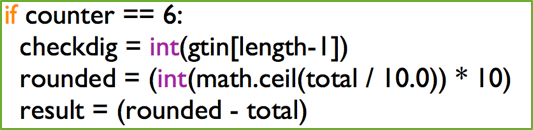
\includegraphics{task1_subtract1.png} ~\par
This snippet checks to see if the loop is on its final iteration (\verb|counter| = 6). It then sets \verb|checkdig| to the penultimate digit of \verb?gtin?. It then creates the variable \verb?rounded? and sets it to to the nearest highest multiple of 10 of \verb?total?. It then creates the variable \verb?result? and sets it to the result of \verb?rounded? - \verb?total?.
\paragraph{Objective 3: Compare this to the given 8th number, or complete the 7-digit number} ~\par ~\par
\noindent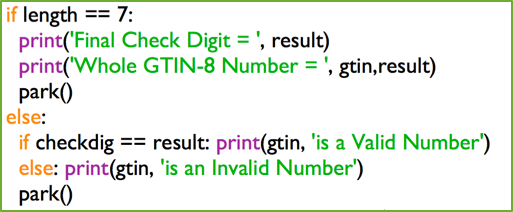
\includegraphics{task1_compare1.png} ~\par
In this section of code, if \verb?length? equals 7, the program prints the final check digit (\verb?result?), and also prints the whole calculated GTIN (\verb?gtin? and \verb?result?). It then calls the \verb|park()| function
Else, if \verb?checkdig? is equal to \verb?result?, it prints that \verb?gtin? is a valid number. Else, it prints that \verb?gtin? is an invalid number.


\subsection{Task 2}




\end{document}
